\documentclass[12pt, twosides]{report}

\usepackage{graphicx}
\graphicspath{ {figures/} }
\usepackage[left=2.5cm,right=2cm,top=2.5cm]{geometry}

%\usepackage{fontspec}
%\setmainfont{Times New Roman}

\usepackage[utf8]{inputenc}
\usepackage{t1enc}
\usepackage[magyar]{babel}
\linespread{1.5}

\usepackage{footnote}
\usepackage{subfigure}
\usepackage{float}
\usepackage[]{algorithm2e}
\usepackage{amsmath}
\usepackage{mathptmx}
\usepackage{pdfpages}

\usepackage{xcolor}
\usepackage{hyperref}
\hypersetup{
    colorlinks,
    linkcolor=black,
    citecolor=black,
	urlcolor={blue!80!black},
	unicode=true
}
% 
\urlstyle{same}

\usepackage{listings}
\definecolor{dkgreen}{rgb}{0,0.6,0}
\definecolor{gray}{rgb}{0.5,0.5,0.5}
\definecolor{mauve}{rgb}{0.58,0,0.82}
\definecolor{light-gray}{gray}{0.25}

\lstdefinestyle{yaml}{	
	backgroundcolor=\color{white}, % choose the background color;
	basicstyle=\fontsize{8}{8}\ttfamily,% the size of the fonts that are used for the code
	breakatwhitespace=false, % sets if automatic breaks should only happen at whitespace
	breaklines=true, % sets automatic line breaking
	commentstyle=\color{dkgreen},  % comment style
	deletekeywords={...},  % if you want to delete keywords from the given language
	escapeinside={\%}{)},  % if you want to add LaTeX within your code
	extendedchars=true,  % lets you use non-ASCII characters; for 8-bits encodings only, does not work with UTF-8
	frame=none,	 	 % adds a frame around the code
	keepspaces=true, % keeps spaces in text, useful for keeping indentation of code (possibly needs columns=flexible)
	keywordstyle=\color{blue}\bfseries, % keyword style
	otherkeywords={*,...}, % if you want to add more keywords to the set
	numbers=none,  % where to put the line-numbers; possible values are (none, left, right)
	numbersep=5pt, % how far the line-numbers are from the code
	numberstyle=\tiny\color{gray}, % the style that is used for the line-numbers
	rulecolor=\color{black}, % if not set, the frame-color may be changed on line-breaks within not-black text (e.g. comments (green here))
	showspaces=false,% show spaces everywhere adding particular underscores; it overrides 'showstringspaces'
	showstringspaces=false,  % underline spaces within strings only
	showtabs=false,  % show tabs within strings adding particular underscores
	%stepnumber=1,  % the step between two line-numbers. If it's 1, each line will be numbered
	stringstyle=\color{mauve}, % string literal style
	tabsize=2,
	columns=fullflexible  % Using fixed column width (for e.g. nice alignment)
	sensitive = true,
	morekeywords={name, runs-on, on, jobs, build, run, steps, uses}
}
\lstset{style=yaml}

\title{
	{Elektronikai alkatrész teszter}\\
	{\large Sapientia\\
	Erdélyi Magyar Tudományegyetem, Marosvásárhely}
}
\author{
	Lukács, Botond\\
	\texttt{lukacs.botond@student.ms.sapientia.ro}
	\and
	dr. Túrós, László-Zsolt\\
	\texttt{turosl@ms.sapientia.ro }	
}
\date{2022}

%%%%%%%%%%%%%%%%%%%%%%%%%%%%%%%%%%%%%%%%%%%%%%%%%%%%%%%%%%%%%%%%%%%%%%%%%
\begin{document}


\includepdf[pages={1,2,3}]{pdfs/allamvizsga_boritoMod.pdf}

\section*{Extras}
Extract

\textbf{Cuvinte cheie}: 

\pagebreak


\includepdf[pages={6}]{pdfs/allamvizsga_boritoMod.pdf}

\section*{Kivonat}
Napjainkban a mikrovezérlős rendszereken sok mindenben megtalálhatóak és
manapság nagy számítási kapacitással rendelkeznek, általánosan
alkalmazhatóak sokféle különböző alkalmazásban. Rengeteg funkciójuk van,
az egyszerű LED kapcsolgatástól kezdve komplex rendszerek automatizálásáig.
Ezen kívül könnyű külső kiegészítő tartozékokat amelyekkel sokkal
szélesebb körben használhatóak.

Ennek hatására a dolgozat célkitűzése egy olyan rendszer kialakítása,
amely képes meghatározni egyszerű elektronikai komponenseket és azok
megközelítő értékét és ezen kívül a lábkiosztását is amennyiben ez
szükséges. Az elektronikában sokféle egyszerű komponenssel találkozhatunk,
mint ellenállások, kondenzátorok, tranzisztorok. Viszont egy áramkör
építésénél jó tudni, hogy az a komponens pontosan mi, ez legfőképpen
igaz a különböző félvezetőkre. Sok esetben az azonosítója lekopott,
vagy nem található adatlap így nehéz beazonosítani, hogy pontosan mi
az a komponens. Erre szolgál az „elektronikai alkatrész teszter” amely
automatikusan meghatározza, vagy kiírja, hogy hibás alkatrész ha nem
ismeri fel vagy sérült a tesztelt alkatrész. A rendszer egy mikrovezérlőt
és egy kijelzőt használ az komponens azonosítására és arról levő adatok
kijelzésére a felhasználó felé. Az azonosítás teljesen automata,
csupán csatlakoztatni kell az ismeretlen komponenst és egy kapcsolót
váltani, vagy automatikusan indulva tápfeszültségre csatlakozáskor.

A dolgozatban a mikrovezérlős alkalmazásokról és azok tervezéséről,
alkatrészek felismeréséről és méréséről lesz szó.

\textbf{Kulcsszavak}: mikrovezérlő
\pagebreak

\section*{Abstract}
Abstract

\textbf{Keywords}: 
\pagebreak

\pagenumbering{gobble}

\tableofcontents

\listoffigures

\chapter{Bevezető}
\pagenumbering{arabic}

A mikrovezérlős rendszerek manapság az életünk minden részében megtalálhatóak, kis méretük, 
alacsony áruk és meglehetősen nagy teljesítményükkel sok mindenre általánosan használhatóak. 
Ez nagyban csökkenti a tervezési költségeket, mivel nem kell egy specifikus logikai áramkört 
kialakítani minden egyes alkalmazási területre, csupán új program kódot kell feltölteni és 
használható egy teljesen más célra.

A mikrovezérlő könnyen összeköthetőek külső eszközökkel amellyel rengeteg mindent meg lehet 
valósítani és bővíteni a lehetőség és szabadon vezérelhetők a GPIO-n (General Purpose Input 
Output) keresztül sok mindent el lehet érni, az egyszerű LED kapcsolgatásától komplex jelek 
generálásáig. Általános esetben a mikrovezérlők csak a legfontosabb részeket tartalmazzák, 
mint az Analog Digital Converter amivel egy analóg jelet alakít egy digitális jellé amit a 
processzor fel tud majd dolgozni, ez legfőképpen azért van, mert nem mindenkinek van szüksége 
mindenre így akinek szüksége van az egyszerűen az külsőleg csatolja hozzá. 

Az összeállított rendszert szabadon lehet vezérelni így automatizálni lehet vele folyamatokat 
amivel egyszerűsíti az emberek dolgát. Viszont nagyban gyorsítja a folyamatok sebességét és 
pontosságát, miközben csökkenti a költségeket, mivel nem kell egy képzett dolgozó irányítsa, 
egy ilyen példa a robotkarok irányítása, lehetséges lenne karok segítségével irányítani, 
viszont ez lassú és költésges, mivel minden robotkar mellé kellene egy munkás aki közel sem 
lenne elég nagy pontosságú. 

Ezen kívűl gyakran használják automatizált tesztelésekre is, mivel egyszerű megismételhető 
teszteket végezni velük, miközben képesek valós időben mérni a rendszer viselkedését. Ennek 
a feladatnak is ez a lényege, az alkatrészek tesztelése egy gyors és automatizált módon. 


\section{Téma meghatározása}

A dolgozat célja egy olyan eszköz tervezése, amit bárki elektronikai ismeret nélkül is egyszerűen 
használni lehet. Sok esetben a feliratok az alkatrészeken nehezen látható, lekopott vagy 
egyszerűen nincs feltüntetve. Ilyen esetben sok segítséget tud nyújtani egy olyan eszköz ami 
gyorsan meg tudja határozni a komponenst és a lábkiosztását is amennyiben ez fontos.

Ez különösen nagy segítséget nyújt kezdőknek akik még kevésbé ismerik az alkatrészeket és az 
adatlapjai meg nagyok és komplexek számukra és a fő információk megjelenítése néhány sorban. 
Haladóknak is nagy segítség, mivel az ellenállást színkódjátról egyszerű meghatározni, viszont 
a teszterrel meg lehet határozni, hogy az alkatrész hibás-e, vagyis ha a tranzisztor kiégett 
akkor az is letesztelhető.

A teszternek 3 teszt terminálja van, ebbe kell az ismeretlen komponenst bekötni és képes 
egyszerű elektronikai komponensek (ellenállás, dióda, tranzisztorok, stb.) automatikus 
felismerését és az adatainak meghatározására. Viszont nem képes bonyolultabb áramkörök 
azonosítására aminek összesen tübb mint 3 lába van.

Megvalósítás során a költégek csökkentése a cél, miközben a pontosság nem csökken nagyban. 
Két verzió is összeállítható, az egyik egyszerű ellenállásokkal és a második egy DAC (Digital 
Analog Converter) segítségével. Mindkettő alkalmas a komponensek meghatározására, viszont az 
ellenállásos verzió nem alkalmas karakterisztika diagramm kirajzolására, viszon sokkal olcsóbb, 
mivel nem használ egy külső DAC-ot.

Mérés eredménye kikerül egy kis kijelzőre és grafikus felületen is megtekinthető amennyiben 
egy számítógéphez van csatolva. Viszont a 2 közül legalább az egyikre szükség van, különben a 
mérés eredménye nem lesz látható. A kijelzőt nem kötelező alkalmazni, viszont annélkül csak 
egy laptop/számítógéphez kapcsolva lehet használni.

Ehhez szükséges egy processzor, viszont manapság a mikrovezérlők nagy számítási kapacitással 
rendelkeznek meglehetősen alacsony áron és néhány ellemállásból és vezetékből otthon is 
összeállítható.

Karakterisztika diagramm kirajzolása is fontos, viszont ez leginkább a tranzisztoroknál 
fontos, mivel az ellenállások lineárins összefüggést mutatnak a feszültség és áramerősség közt 
és a diódák meg magas áram növekedést ami után a feszültésg elérte a nyitó feszültséget.

A rendszer táplálása bármilyen USB csatlakozón keresztül lehetséges, mivel ez széles körben 
megtatlálható vagy külső akkumulátor is megfelel amelynek van USB kimenete.

\section{Hasonló eszközök}

Just \hyperlink{label1}{Click me!}. In the paper \cite{Test00}...



Ez a verzió egy egyszerűsített verzió, viszont ez is képes felismerni a komponenst és meghatározni a paramétereit, viszont kissebb a pontossága és nem képes karakterisztika diagrammot kirajzolására.

A bekötés a következőképpen lehetséges (lásd \ref{fig:basicTesterConnection} ábra).

\begin{figure}
    \centering
    \hfill
    \subfigure[Insbot]{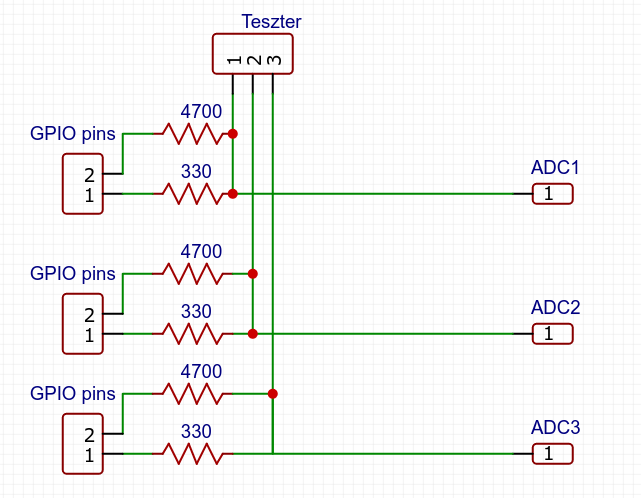
\includegraphics[scale=0.3]{figures/images/literature/BasicTesterConnection.png}}
    \caption{Ellená}
    \label{fig:basicTesterConnection}
\end{figure}



%Két ábra egymás mellett (lásd \ref{fig:insbots} ábra).

%\begin{figure}[h]
%    \centering
%    \hfill
%    \subfigure[Insbot \cite{colot2004insbot}]{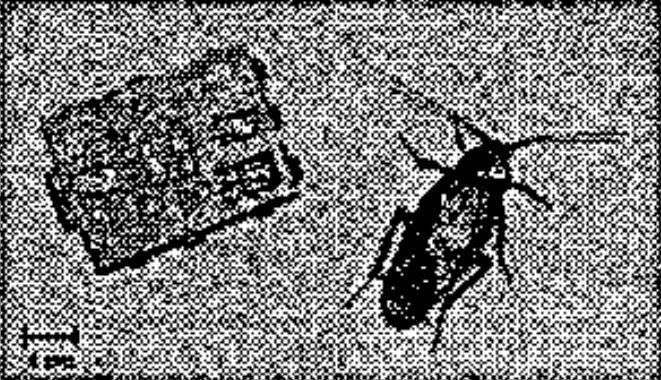
\includegraphics[scale=0.3]{figures/images/literature/insbot.png}}
%    \hfill
%    \subfigure[Insbot és csótányok interakciója \cite{garnier2011ants}.]{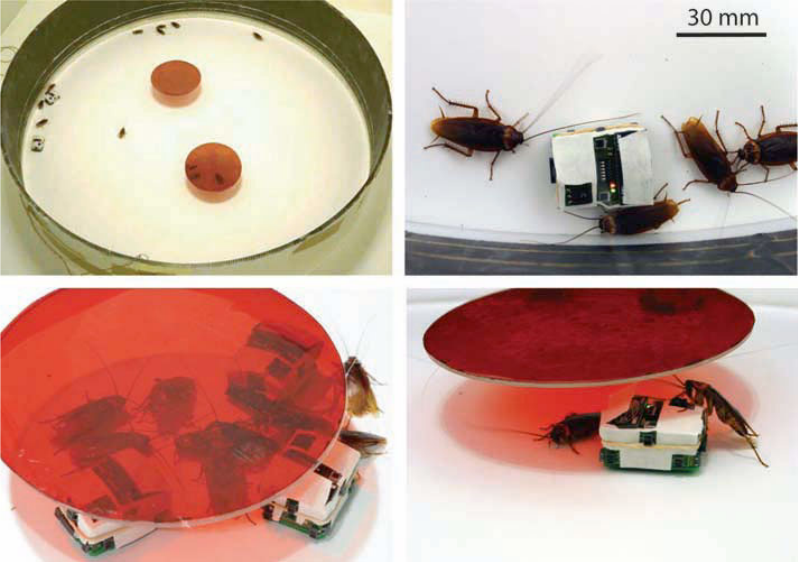
\includegraphics[scale=0.25]{figures/images/literature/insbot_cockroach.png}}
%    
%    \caption{Insbot és csótányok interakciója. Az insbot-ok képesek a csótányokat csalogatni.}
%    \label{fig:insbots}
%\end{figure}

\chapter{Szakirodalom áttekintése}
\section{Cím 1}

\subsection{Alcím 1}

Táblázat: 

\begin{figure}[h]
    \begin{table}[H]
    \begin{footnotesize}
        \begin{center}
            \begin{tabular}{p{2.5cm}|p{3.5cm}|p{4cm}|p{4cm}}
            \textbf{Kritériumok}                    & V\-rep                              & ARGoS  & Gazebo \\
            \hline         
            Ingyenes                            & Igen, van fizetős verzió is         & Igen             & Igen \\
            \hline         
            Absztrakciós szint                  & Valósághű         & Emelkedett absztrakciós szintet ajánl             & Valósághű  \\
            \hline         
            Robotrajokra optimalizált           & Nem optimalizált         & Teljesen optimalizált           & Képes, nagyobb erőforrásigény, mint az ARGOS-nak  \\
            \hline         
            Nyílt forráskódú                    & Igen         & Igen            & Igen  \\
            \hline         
            Támogatott programozási nyelvek     & C/C++, Python, Java, Lua, Matlab, Octave          & C/C++ és Lua             & C/C++  \\
            \hline         
            Valós robotok modelljei             & Igen          & Igen             & Igen  \\
            \end{tabular}
        \end{center}
    \end{footnotesize}
    \end{table}
    \label{table:simulators}
    \caption{V-REP, ARGoS, Gazebo összehasonlítása}
\end{figure}

Hivatkozás a táblázatra: \ref{table:simulators}

\chapter{Elméleti áttekintés}
\section{Elméleti áttekintés}

Pszeudokód: 

\begin{algorithm}[h]
    \begin{small}
    \KwData{Tanulási tényező ($\alpha \in (0, 1])$), $\epsilon > 0$}
    Véletlenszerű érték minden $Q_{1}(s,a)$ és $Q_{2}(s,a)$-nek, kivéve $Q($terminális$, \cdot ) = 0$, $s \in S$, $a \in A$ \;
    \For{minden epizód}{
        S inicalizálása\;
        \Repeat{S terminális állapot}{
        $A \leftarrow$ cselekvés, $S$ állapotban $\epsilon$-greedy szerint $Q_{1}+Q_{2}$ \;
        $A$ cselekedet végrehajtása, R és S' megfigyelése\;
        \eIf{ $50\%$ eséllyel}
            {$Q_{1}(S, A) \leftarrow Q_{1}(S, A) + \alpha [R + \gamma Q_{2}(S', arg\max_{a}Q_{1}(S', a)) - Q_{1}(S, A)]$}
            {$Q_{2}(S, A) \leftarrow Q_{2}(S, A) + \alpha [R + \gamma Q_{1}(S', arg\max_{a}Q_{2}(S', a)) - Q_{2}(S, A)]$}
        $S \leftarrow S'$\;
        }
    }
    \end{small}
    \caption{Dupla Q-tanulás \cite{sutton2018reinforcement}.}        
    \label{algo:double_q}
\end{algorithm}


Hivatkozás pszeudokódra: \ref{algo:double_q}.

\chapter{Rendszer specifikációi}
\section{Cím 1}

%Terv
\chapter{Gyakorlati megvalósítás} \label{chpt:implementation}
\section{Ágensek vezérlése}

\textbf{Hivatkozásra példa}

Az ágensek vezérléséhez a potenciálmező navigációs módszer volt felhasználva. Ez egy bevált módszer a robotrajok vezérléséhez \cite{szanto2015investigation}. Az alapötlete, hogy az akadályok taszító erővel hatnak az ágensre és a cél vonzó erővel. Ennek a két erőnek az eredője határozza meg az irányt amerre érdemes haladni.

\subsection{Potenciálmező navigáció}

\textbf{Egyenletekre példa}

A potenciálmező navigációs módszernél az erők nagysága az \eqref{eq:poti} egyenlet szerint van kiszámolva.

\begin{equation}
    \left\{
    \begin{array}{l}
        |\vec{f}_{push}| = a e ^ {- \frac{(x - b_{push}) ^ {2}}{2 c_{push}^2 }} \\
        |\vec{f}_{pull}| = a e ^ {- \frac{(x - b_{pull}) ^ {2}}{2 c_{pull}^2 }} \\
    \end{array}
    \right.
    \label{eq:poti}
\end{equation}

\begin{itemize}
    \item a: Gauss görbe magassága
    \item b: Gauss görbe középpontja
    \item c: Gauss görbe szélessége
\end{itemize}

\begin{equation}
    \vec{f}_{robot} = \sum_{i} \vec{f}_{push_{i}} + \sum_{i} \vec{f}_{pull_{i}}
    \label{eq:poti_eredo}
\end{equation}

Az eredő vektor a \eqref{eq:poti_eredo} képlet szerint volt kiszámolva. 


\chapter{Eredmények}
\section{Cím 1}

Eredmények leírása

\begin{figure}[h]
    \centering
    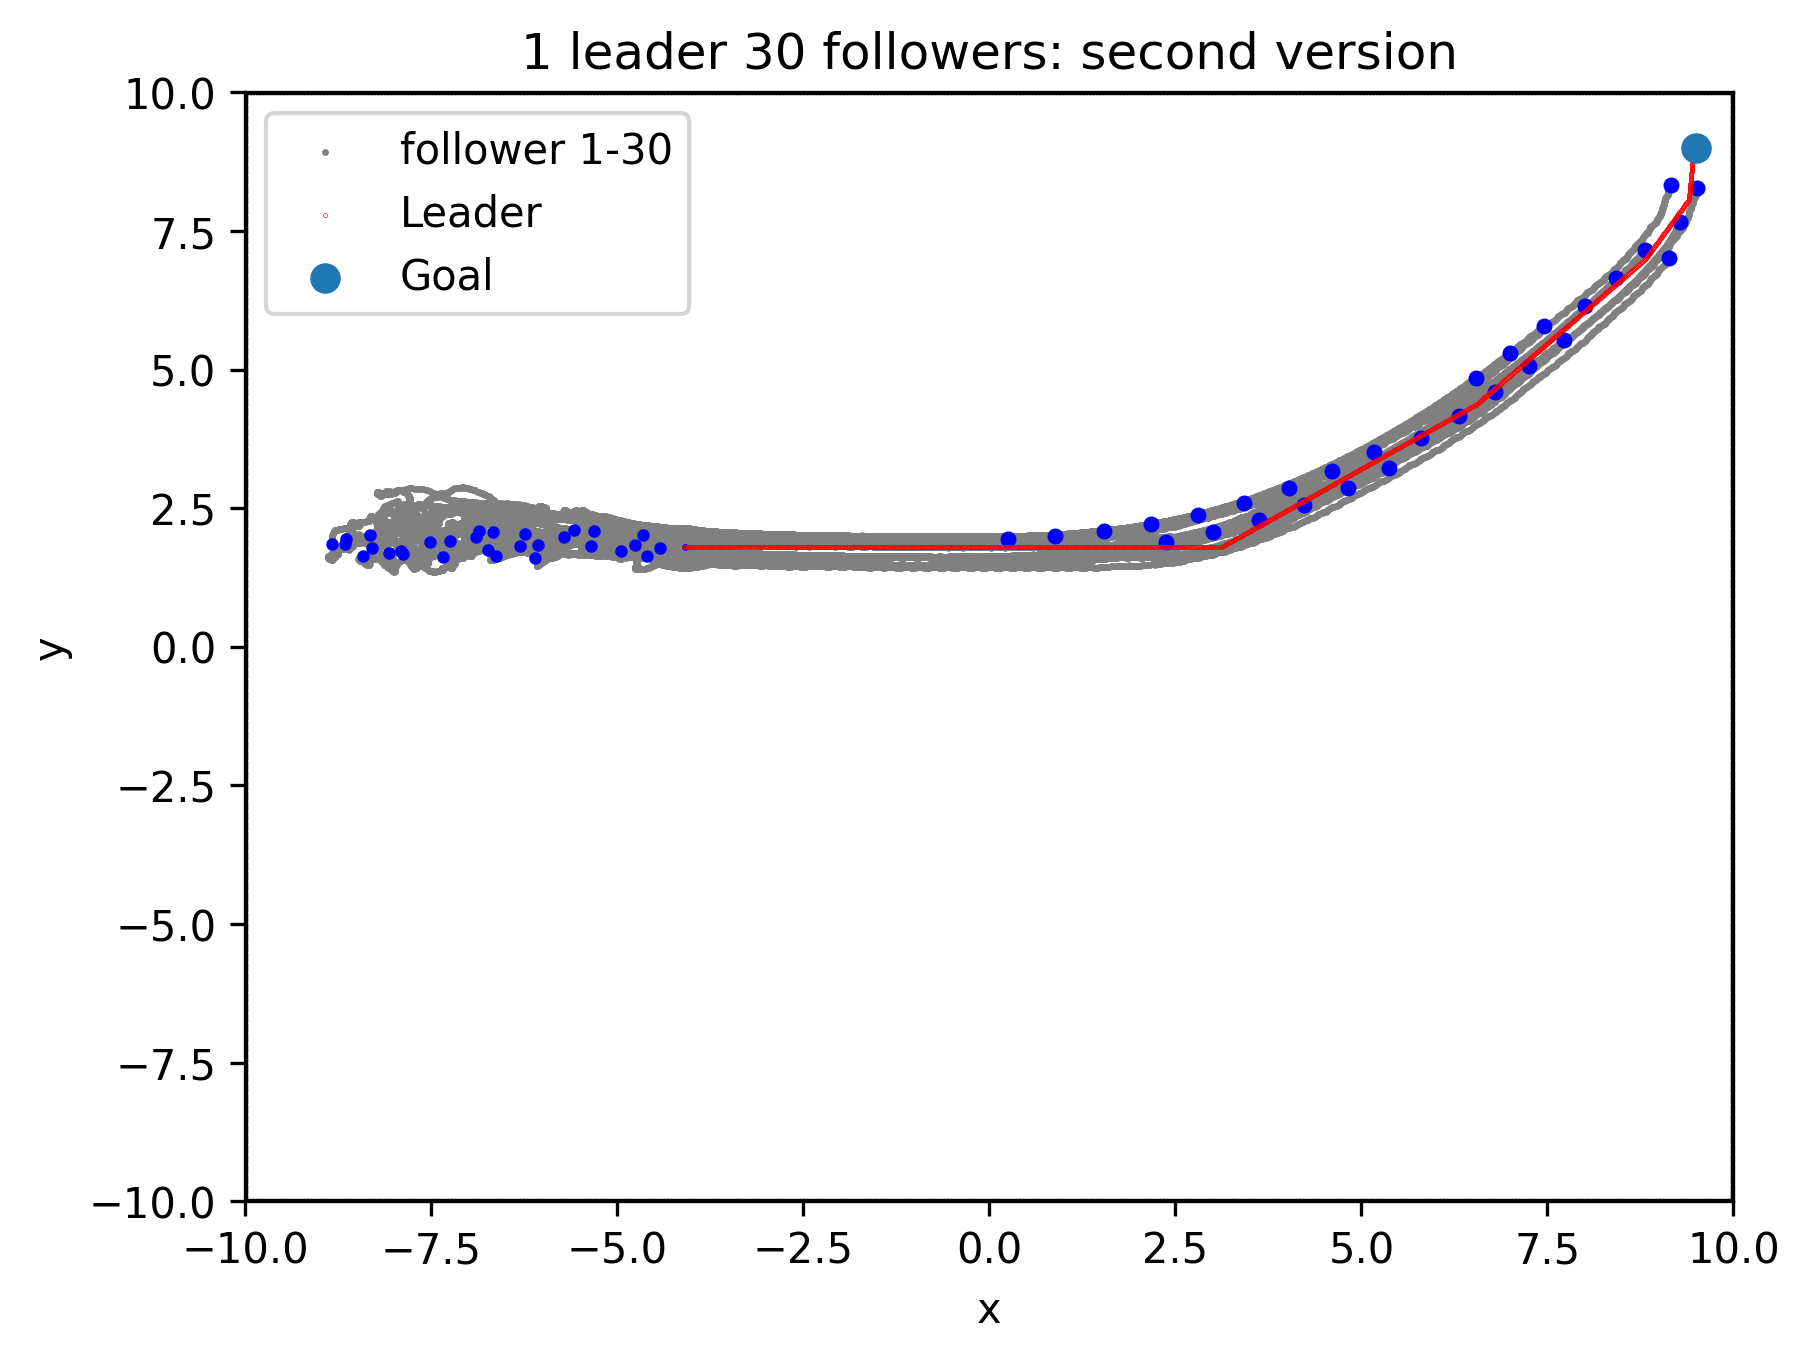
\includegraphics[scale=0.8]{figures/images/results/swarm_second_version.png}
    \caption{30 követő ágens, egy vezér}
    \label{fig:result_30_foll_1_lead}
\end{figure}





%következtetés
\chapter{Összefoglalás}
\section{Összefoglalás}

\addcontentsline{toc}{chapter}{Irodalomjegyzék}
\bibliographystyle{ieeetr}
\bibliography{References}

%appendix
\appendix
\chapter{Függelék}
\section{Alfejezet}

\subsection{Cím}

\subsubsection{Alcím}




\end{document}